\chapter{Ciclos de vida e reprodução das plantas terrestres}\label{ch:b2:plant-life-cycles}

A almofada verde de \omterm{def:b2:plant-life-cycles:moss}{musgo} sobre um muro é uma planta; as hastes
castanhas que se erguem dela na primavera, cada uma com uma cápsula de
esporos, são outra --- um indivíduo diferente, com o dobro de
cromossomos, que cresce a partir do primeiro e vive à custa dele. A
fronde de uma \omterm{def:b2:plant-life-cycles:fern}{samambaia} leva esporos em sua face inferior, mas os
esporos não crescem em \omterm{def:b2:plant-life-cycles:fern}{samambaias}: crescem numa lâmina verde em forma
de coração, de poucos milímetros de largura, onde são produzidos os
anterozoides e as oosferas, e é dessa lâmina que brota uma nova
\omterm{def:b2:plant-life-cycles:fern}{samambaia}. Toda planta terrestre alterna assim entre dois corpos, um
\omterm{def:b2:meiosis-heredity:meiosis}{haploide} e um \omterm{def:b2:meiosis-heredity:meiosis}{diploide}. Este capítulo acompanha essa alternância das
algas até a semente, e mostra como uma sequência de modificações ---
a redução do corpo \omterm{def:b2:meiosis-heredity:meiosis}{haploide}, a invenção do \omterm{def:b2:plant-life-cycles:heterospory}{pólen}, o encerramento do
\omterm{def:b2:plant-life-cycles:heterospory}{óvulo}, a semente --- libertou a reprodução da água e permitiu que as
plantas cobrissem os continentes.

\section{Três tipos de ciclo de vida}

\begin{definition}[Haplonte, diplonte, haplodiplonte]\label{def:b2:plant-life-cycles:cycles}
\index{ciclo de vida}\index{alternância de gerações}\index{gametófito}\index{esporófito}
Todo ciclo de vida sexuado contém uma \emph{fecundação}, que dobra o
número de cromossomos, e uma \emph{\omterm{def:b2:meiosis-heredity:meiosis}{meiose}}, que o reduz à metade; os
ciclos diferem no que acontece entre as duas. Num ciclo
\emph{haplonte}, o zigoto é a única célula \omterm{def:b2:meiosis-heredity:meiosis}{diploide} e sofre \omterm{def:b2:meiosis-heredity:meiosis}{meiose}
imediatamente; o organismo é \omterm{def:b2:meiosis-heredity:meiosis}{haploide} e seus gametas são produzidos
por mitose (\emph{Chlamydomonas}, muitas algas e fungos). Num ciclo
\emph{diplonte}, a \omterm{def:b2:meiosis-heredity:meiosis}{meiose} produz diretamente os gametas, os gametas
são as únicas células \omterm{def:b2:meiosis-heredity:meiosis}{haploides} e o organismo é \omterm{def:b2:meiosis-heredity:meiosis}{diploide} (os animais,
a alga parda \emph{Fucus}). Num ciclo \emph{haplodiplonte}, a \omterm{def:b2:meiosis-heredity:meiosis}{meiose}
produz \emph{esporos}, que crescem por mitose num organismo \omterm{def:b2:meiosis-heredity:meiosis}{haploide},
o \emph{gametófito}, que produz gametas por mitose; o zigoto cresce
por mitose num organismo \omterm{def:b2:meiosis-heredity:meiosis}{diploide}, o \emph{esporófito}, que produz
esporos por \omterm{def:b2:meiosis-heredity:meiosis}{meiose}. Dois corpos \omterm{def:b2:unicellular-diversity:unicellular}{multicelulares} se alternam --- a
\emph{alternância de gerações} ---, e esse é o ciclo de todas as
plantas terrestres e de muitas algas.
\end{definition}

\begin{omfigure}
\begin{tikzpicture}[every node/.style={font=\scriptsize}, >=stealth]
  \foreach \dx/\title/\hap/\dip in {0/{haplonte (\emph{Chlamydomonas})}/{organismo haploide ($n$)}/{zigoto ($2n$)}, 5.2/{diplonte (animais)}/{gametas ($n$)}/{organismo diploide ($2n$)}, 10.4/{haplodiplonte (plantas)}/{gametófito ($n$)}/{esporófito ($2n$)}} {
    \begin{scope}[xshift=\dx cm]
      \node[anchor=south, font=\scriptsize\bfseries] at (2,2.5) {\title};
      \draw[thick, omDef, ->] (0.6,0.4) arc (200:340:1.5 and 1.0);
      \draw[thick, omThm, ->] (3.4,1.4) arc (20:160:1.5 and 1.0);
      \node[omDef, anchor=north] at (2,-0.3) {\hap};
      \node[omThm, anchor=south] at (2,2.05) {\dip};
      \node[anchor=south west] at (3.4,1.05) {fecundação};
      \node[anchor=north east] at (0.55,0.75) {meiose};
    \end{scope}
  }
  % emphasise the dominant phase by thickness of the arcs: draw thicker arcs
  \draw[line width=2.4pt, omDef, ->] (0.6,0.4) arc (200:340:1.5 and 1.0);
  \draw[line width=2.4pt, omThm, ->] (5.2+3.4,1.4) arc (20:160:1.5 and 1.0);
  \draw[line width=2.4pt, omDef, ->] (10.4+0.6,0.4) arc (200:340:1.5 and 1.0);
  \draw[line width=2.4pt, omThm, ->] (10.4+3.4,1.4) arc (20:160:1.5 and 1.0);
\end{tikzpicture}

{\small Três \omterm{def:b2:plant-life-cycles:cycles}{ciclos de vida}. Em azul, a fase \omterm{def:b2:meiosis-heredity:meiosis}{haploide}; em vermelho, a
fase \omterm{def:b2:meiosis-heredity:meiosis}{diploide}; os arcos grossos são os corpos \omterm{def:b2:unicellular-diversity:unicellular}{multicelulares}. Todo
ciclo passa uma vez pela \omterm{def:b2:meiosis-heredity:meiosis}{meiose} e uma vez pela fecundação; eles diferem
em qual fase --- ou ambas --- cresce num organismo.}
\end{omfigure}

\begin{proposition}[O que significa a alternância de gerações]\label{prop:b2:plant-life-cycles:alternation}
Numa planta terrestre, as duas gerações são dois organismos, e não
duas etapas de um só: o \omterm{def:b2:plant-life-cycles:cycles}{gametófito} e o \omterm{def:b2:plant-life-cycles:cycles}{esporófito} têm genomas
diferentes (\omterm{def:b2:meiosis-heredity:meiosis}{haploide} e \omterm{def:b2:meiosis-heredity:meiosis}{diploide}), corpos diferentes, muitas vezes
tamanhos que diferem em ordens de grandeza, e cada um se desenvolve
por mitose a partir de uma única célula --- um esporo ou um zigoto. O
\omterm{def:b2:plant-life-cycles:cycles}{gametófito} produz gametas em órgãos \omterm{def:b2:unicellular-diversity:unicellular}{multicelulares}, os
\emph{\omterm{def:b2:plant-life-cycles:moss}{anterídios}} (anterozoides) e os \emph{\omterm{def:b2:plant-life-cycles:moss}{arquegônios}} (uma oosfera
cada, num frasco por cujo colo o anterozoide desce nadando); o
\omterm{def:b2:plant-life-cycles:cycles}{esporófito} produz esporos em \emph{\omterm{def:b2:plant-life-cycles:fern}{esporângios}}. Ao longo das plantas
terrestres, o equilíbrio se desloca: nos \omterm{def:b2:plant-life-cycles:moss}{musgos}, o \omterm{def:b2:plant-life-cycles:cycles}{gametófito} é a
planta e o \omterm{def:b2:plant-life-cycles:cycles}{esporófito} uma haste dependente; nas \omterm{def:b2:plant-life-cycles:fern}{samambaias}, o
\omterm{def:b2:plant-life-cycles:cycles}{esporófito} é a planta e o \omterm{def:b2:plant-life-cycles:cycles}{gametófito} uma lâmina de vida livre; nas
plantas com sementes, o \omterm{def:b2:plant-life-cycles:cycles}{gametófito} se reduz a poucas células
escondidas nos tecidos do \omterm{def:b2:plant-life-cycles:cycles}{esporófito} --- o grão de \omterm{def:b2:plant-life-cycles:heterospory}{pólen} e o conteúdo
do \omterm{def:b2:plant-life-cycles:heterospory}{óvulo}.
\end{proposition}
\begin{proof}[Evidências]
Hofmeister (1851) fez germinar os esporos de \omterm{def:b2:plant-life-cycles:moss}{musgos}, \omterm{def:b2:plant-life-cycles:fern}{samambaias},
cavalinhas e licopódios, acompanhou o desenvolvimento dos pequenos
corpos verdes que eles produziam, encontrou neles os \omterm{def:b2:plant-life-cycles:moss}{anterídios} e os
\omterm{def:b2:plant-life-cycles:moss}{arquegônios}, e viu o embrião crescer, a partir da oosfera fecundada
dentro do \omterm{def:b2:plant-life-cycles:moss}{arquegônio}, até formar a planta portadora de esporos. Mostrou
em seguida que o \omterm{def:b2:plant-life-cycles:heterospory}{óvulo} de uma conífera contém as mesmas estruturas,
reduzidas --- \omterm{def:b2:plant-life-cycles:moss}{arquegônios} dentro de um tecido que é um \omterm{def:b2:plant-life-cycles:cycles}{gametófito}
retido ---, e que, portanto, \omterm{def:b2:plant-life-cycles:moss}{musgos}, \omterm{def:b2:plant-life-cycles:fern}{samambaias} e plantas com sementes
formam uma única série com um único ciclo. As contagens de cromossomos
que explicaram as duas gerações (Strasburger, 1894) vieram quarenta
anos depois.
\end{proof}

\section{Musgos: o gametófito é a planta}

\begin{definition}[O ciclo de vida dos musgos]\label{def:b2:plant-life-cycles:moss}
\index{musgo}\index{protonema}\index{arquegônio}\index{anterídio}
Um \emph{esporo} de musgo germina num filamento verde ramificado, o
\emph{protonema}, do qual brotam gemas que crescem nos ramos folhosos
--- o \emph{\omterm{def:b2:plant-life-cycles:cycles}{gametófito}}, de poucos centímetros de altura, sem raízes,
xilema ou floema verdadeiros, fixado por rizoides e absorvendo água
por toda a superfície. Nas pontas dos ramos, ele leva os
\emph{anterídios}, que liberam anterozoides biflagelados numa película
de chuva ou de orvalho, e os \emph{arquegônios}, cada um com uma
oosfera na base de um colo; os anterozoides nadam no máximo alguns
centímetros, guiados por atraentes químicos, e fecundam a oosfera no
lugar. O zigoto cresce no \emph{\omterm{def:b2:plant-life-cycles:cycles}{esporófito}}: um pé inserido no
\omterm{def:b2:plant-life-cycles:cycles}{gametófito}, uma haste (a \emph{seta}) e uma \emph{cápsula} na qual a
\omterm{def:b2:meiosis-heredity:meiosis}{meiose} produz dezenas de milhares de esporos, liberados através de um
anel de dentes higroscópicos que se abrem no ar seco. O \omterm{def:b2:plant-life-cycles:cycles}{esporófito} faz
um pouco de fotossíntese, mas é alimentado pelo \omterm{def:b2:plant-life-cycles:cycles}{gametófito} através do
pé e nunca vive sozinho.
\end{definition}

\begin{omfigure}
\begin{tikzpicture}[every node/.style={font=\scriptsize}, >=stealth]
  \node[draw, rounded corners, fill=omDef!12, align=center] (spore) at (0,3) {esporo ($n$)};
  \node[draw, rounded corners, fill=omDef!12, align=center] (proto) at (3.2,3) {protonema};
  \node[draw, rounded corners, fill=omDef!12, align=center] (gam) at (6.6,3) {gametófito folhoso ($n$)\\anterídios e arquegônios};
  \node[draw, rounded corners, fill=omDef!12, align=center] (gametes) at (11.2,3) {anterozoide e oosfera ($n$)};
  \node[draw, rounded corners, fill=omThm!12, align=center] (zyg) at (11.2,0.8) {zigoto ($2n$)};
  \node[draw, rounded corners, fill=omThm!12, align=center] (sporo) at (6.6,0.8) {esporófito ($2n$)\\pé, seta, cápsula};
  \node[draw, rounded corners, fill=omThm!12, align=center] (cap) at (2.4,0.8) {meiose na cápsula};
  \draw[->, thick] (spore) -- (proto) node[midway, above] {mitose};
  \draw[->, thick] (proto) -- (gam);
  \draw[->, thick] (gam) -- (gametes) node[midway, above] {mitose};
  \draw[->, thick] (gametes) -- (zyg) node[pos=0.3, right, align=left] {fecundação\\numa película de água};
  \draw[->, thick] (zyg) -- (sporo) node[midway, above] {mitose};
  \draw[->, thick] (sporo) -- (cap);
  \draw[->, thick] (cap) -| (spore) ;
  \node[omDef, anchor=west] at (-1.9,3.9) {haploide};
  \node[omThm, anchor=west] at (-1.9,-0.1) {diploide};
  \draw[gray, dashed] (-1.9,1.9) -- (13.2,1.9);
\end{tikzpicture}

{\small O ciclo dos \omterm{def:b2:plant-life-cycles:moss}{musgos}. A planta folhosa é o \omterm{def:b2:plant-life-cycles:cycles}{gametófito} \omterm{def:b2:meiosis-heredity:meiosis}{haploide}; o
\omterm{def:b2:plant-life-cycles:cycles}{esporófito} é uma haste com cápsula que cresce sobre ele, alimentado por
ele, e produz esporos por \omterm{def:b2:meiosis-heredity:meiosis}{meiose}.}
\end{omfigure}

\begin{omfigure}
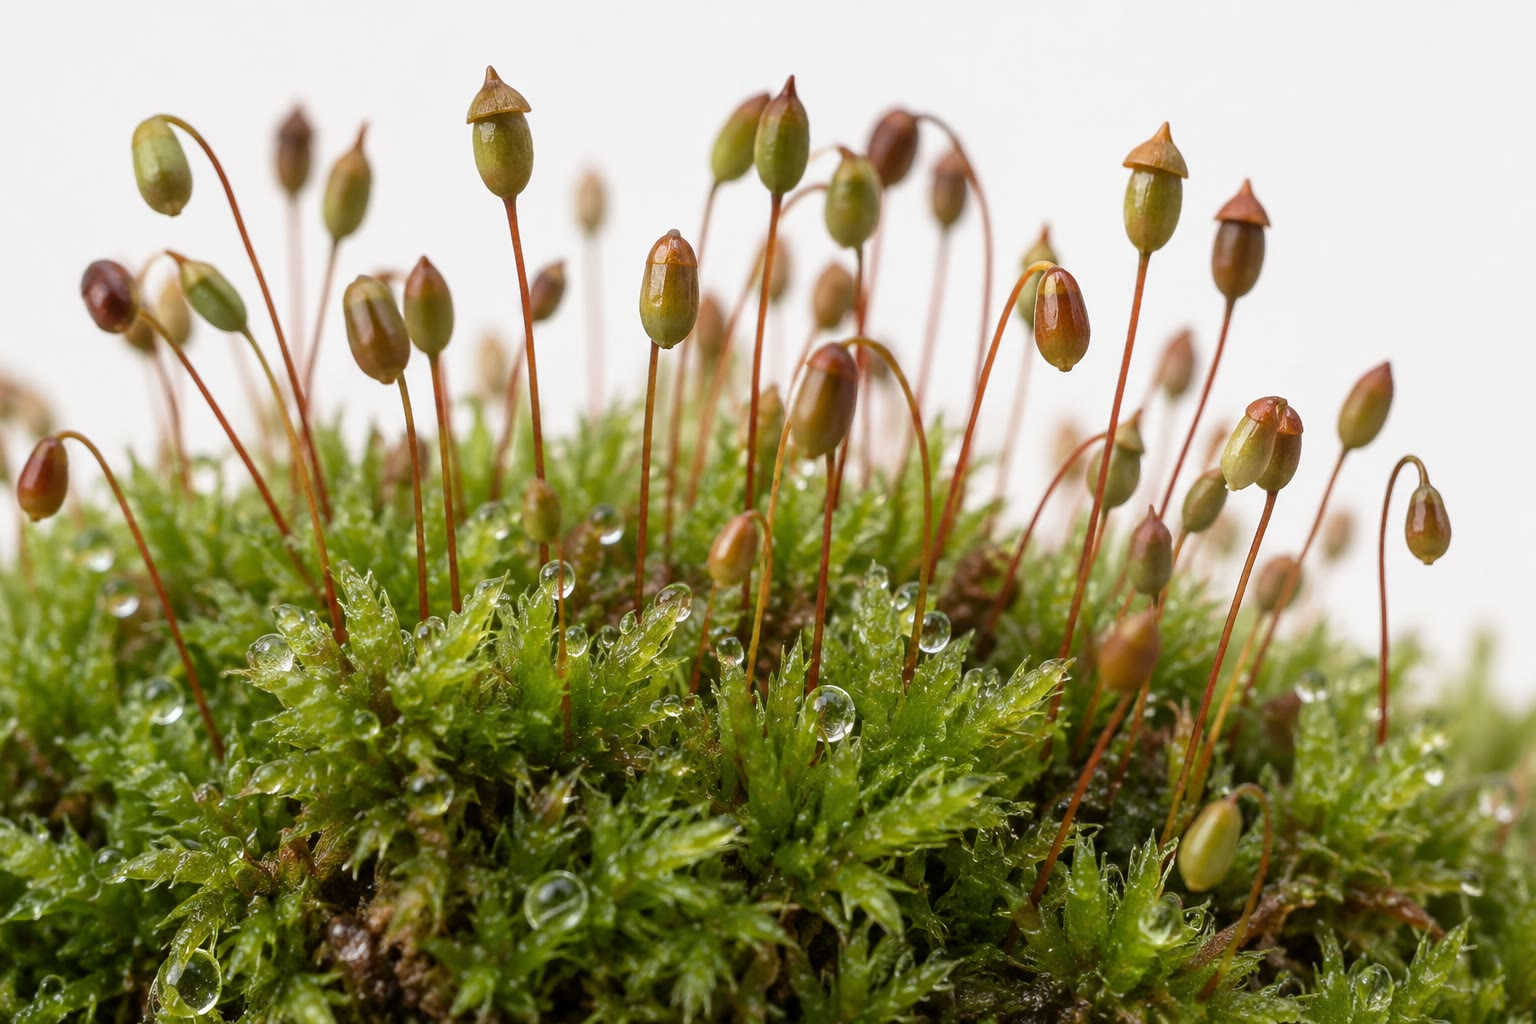
\includegraphics[width=0.6\linewidth]{images/book4/ai/b4-05-moss-sporophytes.jpg}

{\small Uma almofada de \omterm{def:b2:plant-life-cycles:moss}{musgo} na primavera: os ramos verdes são os
\omterm{def:b2:plant-life-cycles:cycles}{gametófitos}, e cada haste avermelhada com sua cápsula é um \omterm{def:b2:plant-life-cycles:cycles}{esporófito}
nascido de uma oosfera fecundada, ainda preso ao ramo que produziu a
oosfera.}
\end{omfigure}

\begin{example}[O custo dos anterozoides nadadores]\label{ex:b2:plant-life-cycles:sperm}
Um anterozoide de \omterm{def:b2:plant-life-cycles:moss}{musgo} nada a cerca de \qty{100}{\micro m/s}; para
alcançar um \omterm{def:b2:plant-life-cycles:moss}{arquegônio} a \qty{2}{cm} de distância, ele precisa de
\qty{200}{s} de película de água contínua --- um respingo de chuva, um
orvalho abundante. A fecundação fica, portanto, restrita ao tempo
úmido e a curtas distâncias, e a maioria dos \omterm{def:b2:plant-life-cycles:moss}{musgos}, das \omterm{def:b2:plant-life-cycles:fern}{samambaias} e
de seus parentes vive em lugares úmidos ou se reproduz na estação
chuvosa; os \omterm{def:b2:plant-life-cycles:moss}{anterídios} de alguns \omterm{def:b2:plant-life-cycles:moss}{musgos} ficam numa taça de respingo
cuja forma lança as gotas de chuva, e os anterozoides que elas levam, a
meio metro. Foi dessa dependência que as plantas com sementes
escaparam.
\end{example}

\section{Samambaias: o esporófito é a planta}

\begin{definition}[O ciclo de vida das samambaias]\label{def:b2:plant-life-cycles:fern}
\index{samambaia}\index{prótalo}\index{soro}\index{esporângio}
A samambaia é o \emph{\omterm{def:b2:plant-life-cycles:cycles}{esporófito}}: um rizoma com raízes, xilema e
floema, e frondes. Na face inferior das frondes férteis, grupos de
\emph{esporângios} (os \emph{soros}, muitas vezes sob uma dobra
protetora) produzem cada um 64 esporos por \omterm{def:b2:meiosis-heredity:meiosis}{meiose} e os lançam pelo
estalo de um anel de células de parede espessa que seca. Um esporo que
cai em solo úmido cresce num \emph{prótalo}: um \omterm{def:b2:plant-life-cycles:cycles}{gametófito} verde em
forma de coração, de poucos milímetros de largura, com uma célula de
espessura, com rizoides, que vive livre por algumas semanas. Ele leva
\omterm{def:b2:plant-life-cycles:moss}{anterídios} e \omterm{def:b2:plant-life-cycles:moss}{arquegônios} em sua face inferior; os anterozoides nadam
na película de água do solo até a oosfera; o zigoto cresce num jovem
\omterm{def:b2:plant-life-cycles:cycles}{esporófito} que tira seu primeiro alimento do prótalo e depois enraíza,
e o prótalo morre. As duas gerações são ambas independentes, mas
desiguais: o \omterm{def:b2:plant-life-cycles:cycles}{esporófito} vive décadas e pode ter metros de altura; o
\omterm{def:b2:plant-life-cycles:cycles}{gametófito}, semanas e milímetros.
\end{definition}

\begin{omfigure}
\begin{tikzpicture}[every node/.style={font=\scriptsize}, >=stealth]
  \node[draw, rounded corners, fill=omThm!12, align=center] (fern) at (0,3) {samambaia, o esporófito ($2n$)\\raízes, rizoma, frondes};
  \node[draw, rounded corners, fill=omThm!12, align=center] (sor) at (5.4,3) {esporângios em soros\\(sob as frondes)};
  \node[draw, rounded corners, fill=omDef!12, align=center] (spore) at (10.4,3) {esporos ($n$)\\64 por esporângio};
  \node[draw, rounded corners, fill=omDef!12, align=center] (pro) at (10.4,0.6) {prótalo ($n$)\\vida livre, milimétrico\\anterídios, arquegônios};
  \node[draw, rounded corners, fill=omDef!12, align=center] (gam) at (5.4,0.6) {anterozoide e oosfera ($n$)};
  \node[draw, rounded corners, fill=omThm!12, align=center] (zyg) at (0,0.6) {zigoto ($2n$), depois\\jovem esporófito\\sobre o prótalo};
  \draw[->, thick] (fern) -- (sor);
  \draw[->, thick] (sor) -- (spore) node[midway, above] {meiose};
  \draw[->, thick] (spore) -- (pro) node[midway, right] {mitose};
  \draw[->, thick] (pro) -- (gam) node[midway, above] {mitose};
  \draw[->, thick] (gam) -- (zyg) node[midway, above, align=center] {fecundação\\(anterozoides nadadores)};
  \draw[->, thick] (zyg) -- (fern) node[midway, right] {mitose};
  \draw[gray, dashed] (7.9,-0.5) -- (7.9,4.0);
  \node[omThm, anchor=south] at (2.7,3.9) {geração diploide};
  \node[omDef, anchor=south] at (10.4,3.9) {geração haploide};
\end{tikzpicture}

{\small O ciclo das \omterm{def:b2:plant-life-cycles:fern}{samambaias}. A planta que chamamos de \omterm{def:b2:plant-life-cycles:fern}{samambaia} é o
\omterm{def:b2:plant-life-cycles:cycles}{esporófito} \omterm{def:b2:meiosis-heredity:meiosis}{diploide}; o \omterm{def:b2:plant-life-cycles:cycles}{gametófito} \omterm{def:b2:meiosis-heredity:meiosis}{haploide} é um \omterm{def:b2:plant-life-cycles:fern}{prótalo} de vida curta
sobre o qual os anterozoides nadam até as oosferas.}
\end{omfigure}

\begin{omfigure}
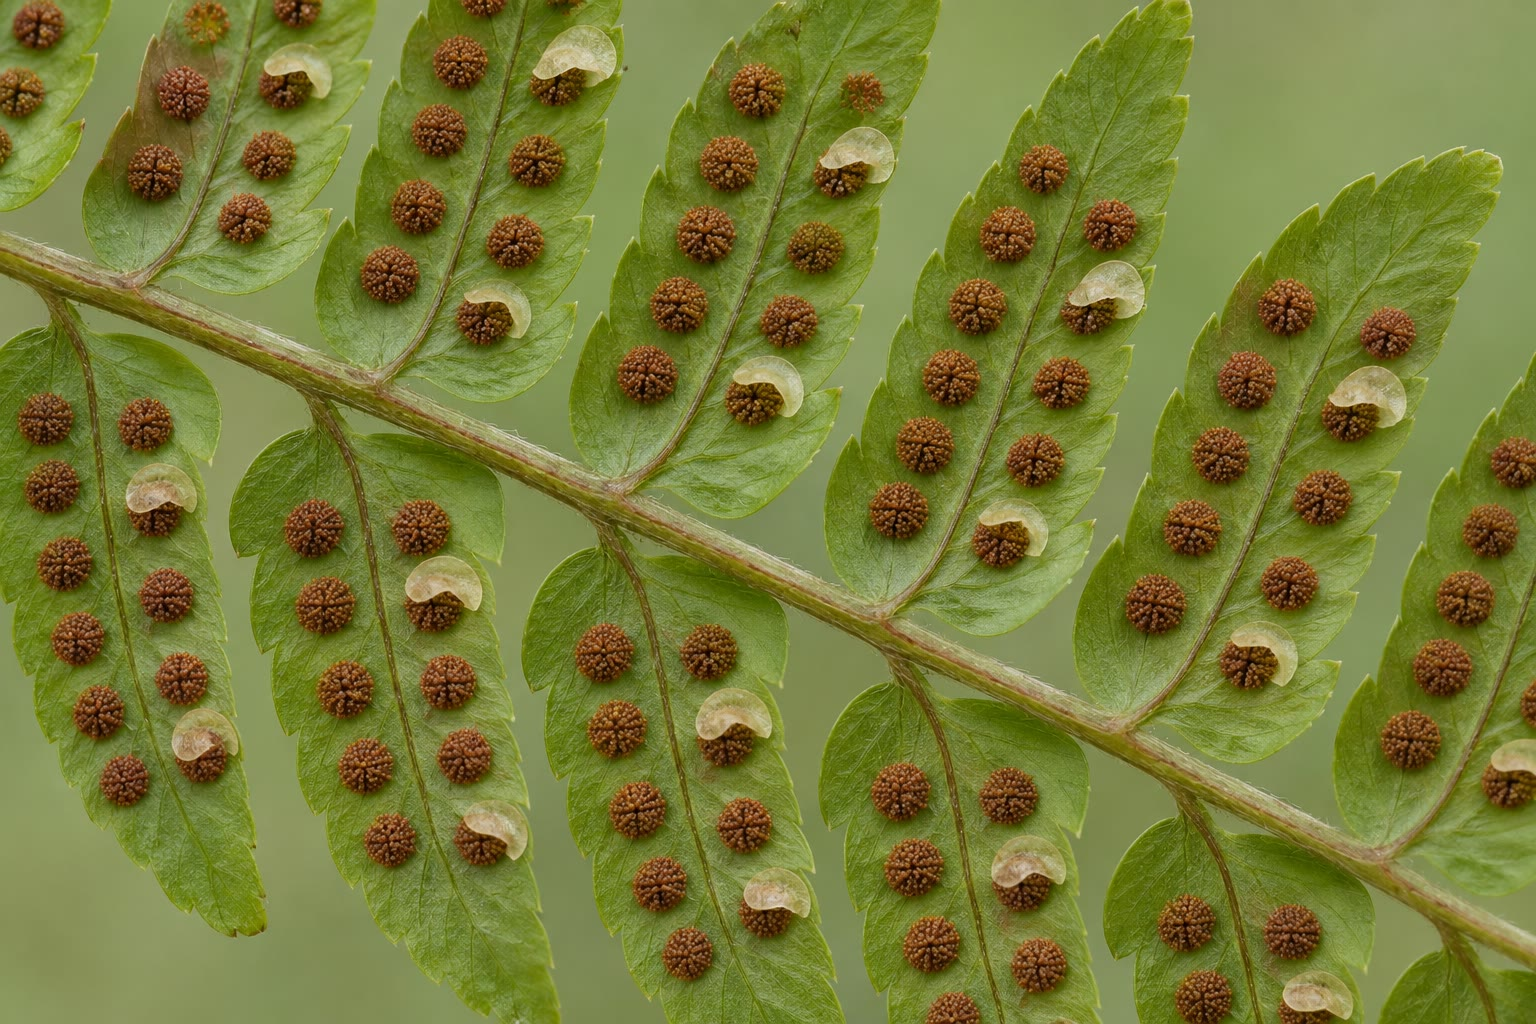
\includegraphics[width=0.6\linewidth]{images/book4/ai/b4-05-fern-sori.jpg}

{\small A face inferior de uma fronde fértil de \omterm{def:b2:plant-life-cycles:fern}{samambaia}: cada ponto
castanho é um \omterm{def:b2:plant-life-cycles:fern}{soro}, um grupo de \omterm{def:b2:plant-life-cycles:fern}{esporângios}, alguns ainda cobertos pela
dobra que os protege até amadurecerem.}
\end{omfigure}

\begin{theorem}[A dispersão de um esporo]\label{thm:b2:plant-life-cycles:dispersal}
\index{dispersão dos esporos}
Um esporo de raio $r$ e densidade $\rho_s$ liberado a uma altura $h$
num vento horizontal de velocidade $u$ cai à velocidade terminal de
Stokes $v_s = 2r^2(\rho_s - \rho_{\text{ar}})g/9\eta_{\text{ar}}$
e pousa, em ar estratificado e calmo, a uma distância
\[
x = \frac{u\,h}{v_s}
\]
da planta. Um esporo de \omterm{def:b2:plant-life-cycles:fern}{samambaia} de raio \qty{15}{\micro m} e
densidade \qty{1100}{kg/m^3} ($\eta_{\text{ar}} = \qty{1.8e-5}{Pa.s}$)
cai a \qty{3}{cm/s}; a partir de uma fronde a \qty{0.5}{m}, num vento
de \qty{2}{m/s}, ele percorre cerca de \qty{30}{m}, e no ar turbulento
de um dia de vento, que eleva uma fração dos esporos muito acima da
altura de liberação, alguns percorrem centenas de quilômetros --- e é
por isso que as floras de \omterm{def:b2:plant-life-cycles:fern}{samambaias} das ilhas oceânicas são ricas e
suas floras de plantas com sementes, pobres.
\end{theorem}
\begin{proof}
O tempo de queda é $h/v_s$ (o esporo atinge sua velocidade terminal em
microssegundos), durante o qual o vento o leva a $u\,h/v_s$. A
velocidade terminal decorre do equilíbrio entre o arrasto de Stokes
$6\pi\eta r
v_s$ e o peso menos o empuxo, $\tfrac43\pi r^3(\rho_s -
\rho_{\text{ar}})g$, como no \cref{ch:b2:unicellular-diversity}.
\end{proof}

\section{Plantas com sementes: o gametófito escondido}

\begin{definition}[Heterosporia, pólen, óvulo]\label{def:b2:plant-life-cycles:heterospory}
\index{heterosporia}\index{pólen}\index{óvulo}\index{micrósporo}\index{megásporo}
Os \omterm{def:b2:plant-life-cycles:moss}{musgos} e a maioria das \omterm{def:b2:plant-life-cycles:fern}{samambaias} são \emph{homospóricos}: um só
tipo de esporo, um só tipo de \omterm{def:b2:plant-life-cycles:cycles}{gametófito}, com os dois sexos. As
plantas com sementes (e algumas \omterm{def:b2:plant-life-cycles:fern}{samambaias} e licopódios) são
\emph{heterospóricas}: os \emph{micrósporos}, pequenos e numerosos,
crescem em \omterm{def:b2:plant-life-cycles:cycles}{gametófitos} masculinos; os \emph{megásporos}, grandes e
poucos, em \omterm{def:b2:plant-life-cycles:cycles}{gametófitos} femininos. Nas plantas com sementes, ambos se
reduzem a quase nada, e nenhum deles deixa por conta própria os
tecidos do \omterm{def:b2:plant-life-cycles:cycles}{esporófito}. O \omterm{def:b2:plant-life-cycles:cycles}{gametófito} masculino é o \emph{grão de
pólen}: um micrósporo que se dividiu duas ou três vezes dentro de sua
parede, levado pelo vento ou por animais até o órgão feminino, onde
forma um \emph{tubo polínico} e entrega seus gametas masculinos ---
sem necessidade de água. O \omterm{def:b2:plant-life-cycles:cycles}{gametófito} feminino se desenvolve dentro do
megasporângio, que permanece na planta-mãe envolto por um ou dois
\emph{tegumentos} com um poro, a \emph{micrópila}: a estrutura inteira
é o \emph{óvulo}. Após a fecundação, o óvulo se torna a
\emph{semente}: um \omterm{def:b2:plant-life-cycles:cycles}{esporófito} embrionário, uma reserva de alimento e
um envoltório formado a partir dos tegumentos, dormente até que as
condições sejam favoráveis.
\end{definition}

\begin{omfigure}
\begin{tikzpicture}[every node/.style={font=\scriptsize}]
  % ovule in section
  \draw[thick, fill=omExo!25] (0,0) ellipse (1.6 and 2.2);
  \draw[thick, fill=omExo!10] (0,0) ellipse (1.25 and 1.85);
  \draw[thick, fill=white] (0,-0.15) ellipse (0.8 and 1.3);
  \draw[thick, fill=omDef!25] (0,0.6) ellipse (0.45 and 0.55);
  \fill[omDef!80!black] (0,0.75) circle (0.12);
  % micropyle: gap at top
  \fill[white] (-0.35,1.7) rectangle (0.35,2.35);
  \draw[thick] (-0.35,1.7) -- (-0.35,2.2); \draw[thick] (0.35,1.7) -- (0.35,2.2);
  \draw[thick] (-0.35,2.2) arc (180:90:0.1) ; \draw[thick] (0.35,2.2) arc (0:90:0.1);
  % pollen grain and tube
  \draw[thick, fill=omProp!40] (0.9,3.0) circle (0.22);
  \draw[thick, omProp] (0.75,2.85) .. controls (0.2,2.6) and (0.05,2.0) .. (0.05,1.25);
  % stalk
  \draw[thick] (0,-2.2) -- (0,-2.8);
  % labels
  \draw (1.45,-0.9) -- (2.6,-0.9) node[right] {tegumento(s)};
  \draw (1.0,-0.6) -- (2.6,-1.5) node[right] {megasporângio (nucelo)};
  \draw (0.55,-1.0) -- (2.6,-2.1) node[right, align=left] {gametófito feminino\\(de um megásporo)};
  \draw (0.35,0.45) -- (2.6,0.3) node[right] {arquegônio};
  \draw (0.1,0.78) -- (2.6,1.0) node[right] {oosfera};
  \draw (0.35,2.0) -- (2.6,2.0) node[right] {micrópila};
  \draw (1.1,3.0) -- (2.6,3.0) node[right] {grão de pólen e tubo polínico};
  \node[right] at (0.1,-2.6) {pedúnculo};
\end{tikzpicture}

{\small \omterm{def:b2:plant-life-cycles:heterospory}{Óvulo} de gimnosperma em corte. O \omterm{def:b2:plant-life-cycles:cycles}{gametófito} feminino, formado a
partir de um único \omterm{def:b2:plant-life-cycles:heterospory}{megásporo} dentro do megasporângio, é envolto por um
tegumento com um poro; o grão de \omterm{def:b2:plant-life-cycles:heterospory}{pólen}, retido na micrópila, forma um
tubo até a oosfera. Após a fecundação, o conjunto se torna a semente.}
\end{omfigure}

\begin{proposition}[O ciclo das coníferas]\label{prop:b2:plant-life-cycles:conifer}
\index{conífera}\index{cone}\index{semente}
Um pinheiro tem dois tipos de cone. Os pequenos \emph{cones
masculinos}, em cachos na primavera, contêm microsporângios nos quais a
\omterm{def:b2:meiosis-heredity:meiosis}{meiose} produz \omterm{def:b2:plant-life-cycles:heterospory}{micrósporos}; cada um se divide num grão de \omterm{def:b2:plant-life-cycles:heterospory}{pólen} de
quatro células com dois sacos aéreos e é liberado aos milhões no
vento. Os \emph{cones femininos} têm dois \omterm{def:b2:plant-life-cycles:heterospory}{óvulos} na face superior de
cada escama. O \omterm{def:b2:plant-life-cycles:heterospory}{pólen} soprado entre as escamas é atraído para a
micrópila por uma gota de líquido; o \omterm{def:b2:plant-life-cycles:cycles}{gametófito} feminino, que ainda
não se desenvolveu, cresce então ao longo do ano seguinte, a partir do
único \omterm{def:b2:plant-life-cycles:heterospory}{megásporo} sobrevivente, até formar um tecido de alguns milhares
de células com dois ou três \omterm{def:b2:plant-life-cycles:moss}{arquegônios}; um tubo polínico cresce
lentamente através do nucelo e, quinze meses após a polinização,
entrega um gameta masculino a uma oosfera. O embrião se desenvolve no
\omterm{def:b2:plant-life-cycles:cycles}{gametófito}, que se torna a reserva de alimento da semente; a semente,
alada, é liberada no segundo outono, quando o cone se abre. As
sementes levam anos e custam caro; em troca, são dispersadas secas,
sobrevivem ao inverno e à seca, e levam o alimento das primeiras
semanas da plântula.
\end{proposition}

\begin{omfigure}
\begin{tikzpicture}[every node/.style={font=\scriptsize}, >=stealth]
  \draw[thick, ->] (0,0) -- (13.2,0);
  \foreach \x/\l in {0/{primavera, ano 1}, 4.4/{primavera, ano 2}, 8.8/{outono, ano 2}, 12.4/{}}
    \draw (\x,0.1) -- (\x,-0.1) node[below] {\l};
  \node[above, align=center, omProp] at (0.6,0.3) {polinização:\\pólen retido na micrópila};
  \node[above, align=center, omDef] at (3.0,1.2) {o gametófito feminino cresce\\a partir do megásporo (um ano)};
  \draw[omDef, thick] (0.8,1.15) -- (5.2,1.15);
  \node[above, align=center, omThm] at (5.6,0.3) {fecundação:\\o tubo polínico chega à oosfera};
  \node[above, align=center, omThm] at (8.2,1.2) {o embrião se desenvolve\\dentro do gametófito};
  \draw[omThm, thick] (5.8,1.15) -- (10.4,1.15);
  \node[above, align=center] at (10.8,0.3) {o cone se abre:\\sementes aladas liberadas};
\end{tikzpicture}

{\small O calendário de uma semente de pinheiro: polinização na
primeira primavera, fecundação mais de um ano depois, semente liberada
no segundo outono --- cerca de dezoito meses do \omterm{def:b2:plant-life-cycles:heterospory}{pólen} à semente.}
\end{omfigure}

\begin{omfigure}
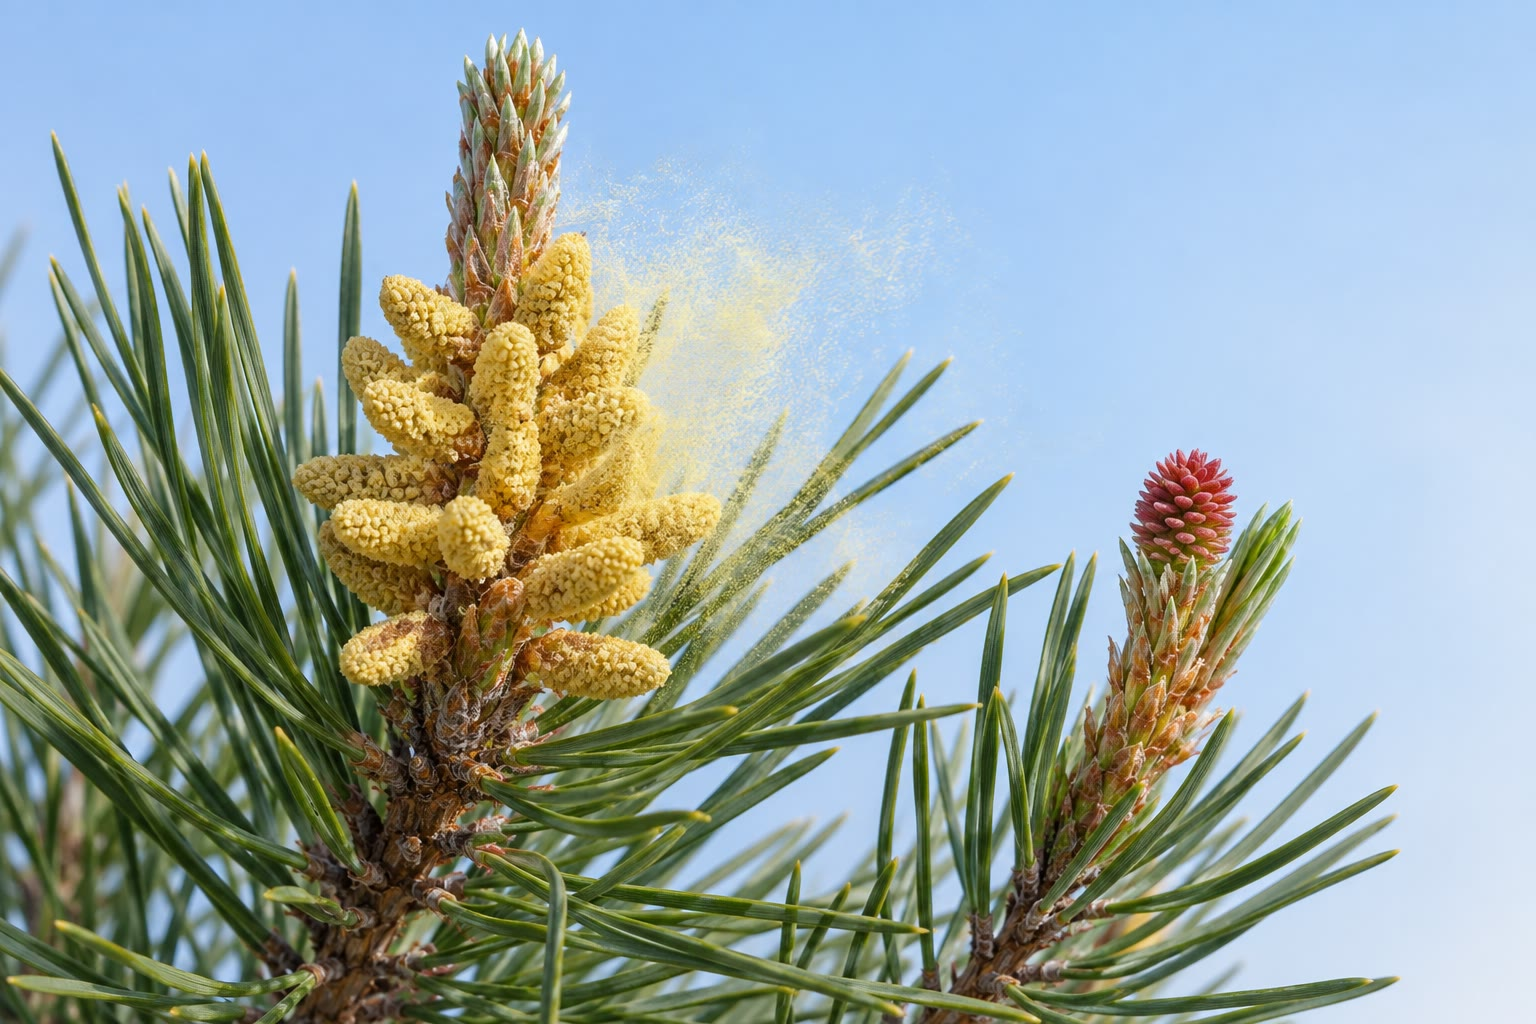
\includegraphics[width=0.6\linewidth]{images/book4/ai/b4-05-pine-cones.jpg}

{\small Um ramo de pinheiro na primavera: um cacho de cones masculinos
amarelos liberando \omterm{def:b2:plant-life-cycles:heterospory}{pólen} e um pequeno cone feminino vermelho na ponta
de outro ramo, com as escamas abertas para captá-lo.}
\end{omfigure}

\begin{example}[O pólen no vento]\label{ex:b2:plant-life-cycles:pollen}
Um grão de \omterm{def:b2:plant-life-cycles:heterospory}{pólen} de pinheiro, de \qty{50}{\micro m} de diâmetro, com
dois sacos aéreos, cai a cerca de \qty{3}{cm/s}; uma árvore grande
libera cerca de $10^{11}$ grãos numa estação, o bastante para cobrir
os lagos de amarelo. A chance de que um grão pouse num dado \omterm{def:b2:plant-life-cycles:heterospory}{óvulo} é
minúscula, e a estratégia só funciona pelo número: a polinização pelo
vento é barata por grão, cara em grãos, e restrita a plantas que
crescem em populações densas de sua própria espécie --- coníferas,
gramíneas, carvalhos. As plantas com flores
(\cref{ch:b2:angiosperm-reproduction}) encontraram um modo de fazer os animais
entregarem o \omterm{def:b2:plant-life-cycles:heterospory}{pólen}, um grão de cada vez, no endereço certo.
\end{example}

\section{Tendências ao longo das plantas terrestres}

\begin{proposition}[Quatro tendências]\label{prop:b2:plant-life-cycles:trends}
\index{redução do gametófito}
Dos \omterm{def:b2:plant-life-cycles:moss}{musgos} às \omterm{def:b2:plant-life-cycles:fern}{samambaias} e às plantas com sementes: (1) o \omterm{def:b2:plant-life-cycles:cycles}{esporófito}
passa de uma haste dependente à planta inteira, e o \omterm{def:b2:plant-life-cycles:cycles}{gametófito} encolhe
da planta a uma lâmina e a poucas células; (2) a homosporia dá lugar
à \omterm{def:b2:plant-life-cycles:heterospory}{heterosporia}, e o \omterm{def:b2:plant-life-cycles:cycles}{gametófito} feminino permanece na planta-mãe;
(3) a fecundação passa de anterozoides nadando na água superficial a
um tubo polínico, de modo que a reprodução deixa de depender da chuva;
(4) a unidade de dispersão passa do esporo --- uma única célula com
reservas para um dia --- à semente, um embrião com alimento e
envoltório, capaz de esperar. A geração \omterm{def:b2:meiosis-heredity:meiosis}{diploide} é favorecida em terra
porque um corpo \omterm{def:b2:meiosis-heredity:meiosis}{diploide} mascara as \omterm{def:b2:genome-diversification:mutation}{mutações} recessivas, pode crescer
mais e viver mais tempo com um sistema vascular, e porque um esporo
produzido por \omterm{def:b2:meiosis-heredity:meiosis}{meiose} num \omterm{def:b2:plant-life-cycles:cycles}{esporófito} alto viaja mais longe que um
gameta nadando a partir de um \omterm{def:b2:plant-life-cycles:cycles}{gametófito} rasteiro. A tendência
continua nas plantas com flores, em que o \omterm{def:b2:plant-life-cycles:cycles}{gametófito} feminino tem sete
células e a semente é envolta por um fruto.
\end{proposition}

\begin{example}[Comparação dos grupos]\label{ex:b2:plant-life-cycles:table}
\begin{center}
\small
\begin{tabular}{p{2.3cm}p{3.1cm}p{3.1cm}p{3.3cm}}
\hline
 & \omterm{def:b2:plant-life-cycles:moss}{musgos} & \omterm{def:b2:plant-life-cycles:fern}{samambaias} & coníferas \\
\hline
geração dominante & \omterm{def:b2:plant-life-cycles:cycles}{gametófito} & \omterm{def:b2:plant-life-cycles:cycles}{esporófito} & \omterm{def:b2:plant-life-cycles:cycles}{esporófito} \\
\omterm{def:b2:plant-life-cycles:cycles}{gametófito} & ramo folhoso, cm & \omterm{def:b2:plant-life-cycles:fern}{prótalo}, mm, livre & grão de \omterm{def:b2:plant-life-cycles:heterospory}{pólen} (4 células); conteúdo do \omterm{def:b2:plant-life-cycles:heterospory}{óvulo} (milhares de células) \\
esporos & um tipo & um tipo & \omterm{def:b2:plant-life-cycles:heterospory}{micrósporos}, \omterm{def:b2:plant-life-cycles:heterospory}{megásporos} \\
fecundação & anterozoides nadam na água & anterozoides nadam na água & tubo polínico \\
unidade de dispersão & esporo & esporo & semente \\
tecido vascular & nenhum & xilema, floema & xilema, floema, madeira \\
\hline
\end{tabular}
\end{center}
\end{example}

\section{Exercícios}

\begin{exercise}[$\star$]\label{exo:b2:plant-life-cycles:1}
Defina \omterm{def:b2:plant-life-cycles:cycles}{gametófito}, \omterm{def:b2:plant-life-cycles:cycles}{esporófito}, esporo e gameta, e diga por qual tipo de
divisão (mitose ou \omterm{def:b2:meiosis-heredity:meiosis}{meiose}) cada um dos quatro é produzido.
\end{exercise}

\begin{exercise}[$\star$]\label{exo:b2:plant-life-cycles:2}
A \omterm{def:b2:plant-life-cycles:fern}{samambaia} \emph{Ophioglossum reticulatum} tem \num{1260}
cromossomos nas células de suas folhas. Quantos há num esporo, numa
célula do \omterm{def:b2:plant-life-cycles:fern}{prótalo}, num anterozoide, numa oosfera, num zigoto?
\end{exercise}

\begin{exercise}[$\star$]\label{exo:b2:plant-life-cycles:3}
Que geração é a almofada verde de um \omterm{def:b2:plant-life-cycles:moss}{musgo}? A haste castanha com uma
cápsula? Uma fronde de \omterm{def:b2:plant-life-cycles:fern}{samambaia}? Um \omterm{def:b2:plant-life-cycles:fern}{prótalo}? Um grão de \omterm{def:b2:plant-life-cycles:heterospory}{pólen}? A
reserva de alimento de uma semente de pinheiro? O embrião de uma
semente de pinheiro?
\end{exercise}

\begin{exercise}[$\star$]\label{exo:b2:plant-life-cycles:4}
Cite os três tipos de \omterm{def:b2:plant-life-cycles:cycles}{ciclo de vida} e dê um organismo para cada um.
Onde ocorre a \omterm{def:b2:meiosis-heredity:meiosis}{meiose} em cada um deles?
\end{exercise}

\begin{exercise}[$\star\star$]\label{exo:b2:plant-life-cycles:5}
Um anterozoide de \omterm{def:b2:plant-life-cycles:moss}{musgo} nada a \qty{100}{\micro m/s}. Quanto tempo ele
leva para alcançar um \omterm{def:b2:plant-life-cycles:moss}{arquegônio} a \qty{3}{cm}? Uma película de
orvalho evapora \qty{20}{min} após o nascer do sol: qual é o alcance
máximo da fecundação? Comente o tamanho das colônias de \omterm{def:b2:plant-life-cycles:moss}{musgo}.
\end{exercise}

\begin{exercise}[$\star\star$]\label{exo:b2:plant-life-cycles:6}
Calcule a velocidade de sedimentação no ar de um esporo de \omterm{def:b2:plant-life-cycles:fern}{samambaia} de
raio \qty{15}{\micro m} e densidade \qty{1100}{kg/m^3} ($\eta =
\qty{1.8e-5}{Pa.s}$, $\rho_{\text{ar}} = \qty{1.2}{kg/m^3}$), e a
distância que ele percorre a partir de \qty{0.5}{m} num vento de
\qty{2}{m/s}. Refaça o cálculo para uma semente de pinheiro de massa
\qty{5}{mg} cuja asa lhe dá uma velocidade de descida de
\qty{0.8}{m/s}, liberada a \qty{20}{m}.
\end{exercise}

\begin{exercise}[$\star\star$]\label{exo:b2:plant-life-cycles:7}
Uma fronde de \omterm{def:b2:plant-life-cycles:fern}{samambaia} leva \num{200} \omterm{def:b2:plant-life-cycles:fern}{soros} de \num{40} \omterm{def:b2:plant-life-cycles:fern}{esporângios},
e cada \omterm{def:b2:plant-life-cycles:fern}{esporângio} produz \num{64} esporos. Quantos esporos há por
fronde? Se um esporo em $10^{5}$ se torna um \omterm{def:b2:plant-life-cycles:fern}{prótalo} e um \omterm{def:b2:plant-life-cycles:fern}{prótalo} em
\num{50} produz um \omterm{def:b2:plant-life-cycles:cycles}{esporófito}, quantas \omterm{def:b2:plant-life-cycles:fern}{samambaias} jovens uma fronde
produz?
\end{exercise}

\begin{exercise}[$\star\star$]\label{exo:b2:plant-life-cycles:8}
Explique por que a \omterm{def:b2:plant-life-cycles:heterospory}{heterosporia} é uma condição prévia para a semente, e
por que uma planta homospórica não poderia encerrar seu \omterm{def:b2:plant-life-cycles:cycles}{gametófito}
feminino num \omterm{def:b2:plant-life-cycles:heterospory}{óvulo}.
\end{exercise}

\begin{exercise}[$\star\star$]\label{exo:b2:plant-life-cycles:9}
Compare um esporo de \omterm{def:b2:plant-life-cycles:fern}{samambaia} (uma esfera de raio \qty{15}{\micro m},
densidade \qty{1100}{kg/m^3}) e uma semente de pinheiro (\qty{5}{mg})
como unidades de dispersão: massa, conteúdo energético (considere
\qty{20}{kJ/g} de matéria seca, \qty{50}{\%} de matéria seca) e o que
cada um pode e não pode fazer ao pousar.
\end{exercise}

\begin{exercise}[$\star\star\star$]\label{exo:b2:plant-life-cycles:10}
Um pinheiro libera $10^{11}$ grãos de \omterm{def:b2:plant-life-cycles:heterospory}{pólen} sobre uma floresta; na
altura dos \omterm{def:b2:plant-life-cycles:heterospory}{óvulos}, os grãos se espalham numa camada de \qty{20}{m} de
espessura sobre \qty{1}{km^2}. Estime a concentração de \omterm{def:b2:plant-life-cycles:heterospory}{pólen} (grãos
por metro cúbico), o número de grãos por segundo que passam pela
abertura micropilar de um \omterm{def:b2:plant-life-cycles:heterospory}{óvulo} (\qty{0.1}{mm^2}) num vento de
\qty{2}{m/s} e o tempo para que um \omterm{def:b2:plant-life-cycles:heterospory}{óvulo} receba um grão. O que isso
diz sobre o momento da abertura dos cones?
\end{exercise}

\begin{exercise}[$\star\star\star$]\label{exo:b2:plant-life-cycles:11}
Dê três razões pelas quais a geração \omterm{def:b2:meiosis-heredity:meiosis}{diploide} passou a dominar o \omterm{def:b2:plant-life-cycles:cycles}{ciclo
de vida} das plantas terrestres, e uma razão pela qual a geração
\omterm{def:b2:meiosis-heredity:meiosis}{haploide} não desapareceu de todo.
\end{exercise}

\begin{exercise}[$\star\star\star$]\label{exo:b2:plant-life-cycles:12}
Hofmeister trabalhou antes de os cromossomos serem conhecidos. Explique
o que ele podia e o que não podia estabelecer sobre a \omterm{def:b2:plant-life-cycles:cycles}{alternância de
gerações} apenas por microscopia e cultivo, e o que as contagens de
cromossomos acrescentaram.
\end{exercise}

\section{Problema: Do esporo à semente}

\begin{problem}[{Problema de fim de semana --- a aritmética reprodutiva
de uma samambaia e de um pinheiro comparada, do número de esporos e de
grãos de pólen à sua dispersão, ao destino dos gametófitos e ao custo
de uma semente, até o número de propágulos que cada planta precisa
produzir para uma substituição}]
\label{pb:b2:plant-life-cycles:1}
Uma \omterm{def:b2:plant-life-cycles:fern}{samambaia} tem \num{10} frondes férteis, cada uma com \num{200}
\omterm{def:b2:plant-life-cycles:fern}{soros} de \num{40} \omterm{def:b2:plant-life-cycles:fern}{esporângios} que produzem \num{64} esporos cada.
Esporos: raio \qty{15}{\micro m}, densidade \qty{1100}{kg/m^3}. Um
pinheiro produz, ao longo da vida, \omterm{def:b2:plant-life-cycles:heterospory}{óvulos} equivalentes a
$2\times 10^{4}$ cones femininos --- considere \num{100} \omterm{def:b2:plant-life-cycles:heterospory}{óvulos} por
cone --- e $10^{11}$ grãos de \omterm{def:b2:plant-life-cycles:heterospory}{pólen} por ano. Sementes: \qty{5}{mg},
\qty{50}{\%} de matéria seca a
\qty{20}{kJ/g}. Ar: $\eta = \qty{1.8e-5}{Pa.s}$, $\rho =
\qty{1.2}{kg/m^3}$; $g = \qty{9.81}{m/s^2}$.

\medskip
\noindent\textbf{Parte I --- Os esporos da \omterm{def:b2:plant-life-cycles:fern}{samambaia}.}
\begin{enumerate}
  \item Calcule o número de esporos que a planta libera numa estação.
  \item Calcule a massa de um esporo e a da produção inteira.
  \item Calcule a velocidade de sedimentação do esporo no ar.
  \item A partir de frondes a \qty{0.5}{m}, num vento de
        \qty{1.5}{m/s}, que distância os esporos percorrem? Sobre que
        área (um disco com esse raio) eles se espalham, e quantos
        pousam por metro quadrado?
  \item Explique por que a turbulência leva alguns esporos muito mais
        longe, e o que isso implica para a colonização de uma ilha nova.
  \item Calcule o conteúdo energético de um esporo (\qty{50}{\%} de
        matéria seca a \qty{20}{kJ/g}) e o da produção inteira, e
        compare com a energia de uma semente de pinheiro.
\end{enumerate}

\medskip
\noindent\textbf{Parte II --- Os \omterm{def:b2:plant-life-cycles:cycles}{gametófitos}.}
Um esporo em $2\times 10^{4}$ pousa num solo úmido o bastante para
crescer num \omterm{def:b2:plant-life-cycles:fern}{prótalo}; um \omterm{def:b2:plant-life-cycles:fern}{prótalo} vive \num{6} semanas e precisa de uma
noite úmida --- probabilidade $0.2$ por semana --- para a fecundação;
um \omterm{def:b2:plant-life-cycles:fern}{prótalo} fecundado dá um jovem \omterm{def:b2:plant-life-cycles:cycles}{esporófito} com probabilidade
$0.5$; um jovem \omterm{def:b2:plant-life-cycles:cycles}{esporófito} sobrevive até a idade adulta com
probabilidade $0.02$.
\begin{enumerate}[resume]
  \item Quantos \omterm{def:b2:plant-life-cycles:fern}{prótalos} a produção da planta gera?
  \item Calcule a probabilidade de que um \omterm{def:b2:plant-life-cycles:fern}{prótalo} tenha pelo menos uma
        noite úmida em suas seis semanas.
  \item Calcule o número esperado de \omterm{def:b2:plant-life-cycles:fern}{samambaias} adultas produzidas pela
        produção de uma estação.
  \item Se a planta-mãe vive \num{30} anos, quantos descendentes
        adultos ela deixa, e o que isso diz sobre a população de
        \omterm{def:b2:plant-life-cycles:fern}{samambaias}?
  \item Um anterozoide de \omterm{def:b2:plant-life-cycles:fern}{samambaia} nada a \qty{100}{\micro m/s}, e os \omterm{def:b2:plant-life-cycles:moss}{arquegônios} de um \omterm{def:b2:plant-life-cycles:fern}{prótalo} ficam a \qty{1}{mm} de
        seus próprios \omterm{def:b2:plant-life-cycles:moss}{anterídios}. Quanto tempo leva a autofecundação?
        Por que muitas \omterm{def:b2:plant-life-cycles:fern}{samambaias} a evitam mesmo assim (dê um
        mecanismo)?
  \item Em que sentido o \omterm{def:b2:plant-life-cycles:fern}{prótalo} é o elo fraco do ciclo das
        \omterm{def:b2:plant-life-cycles:fern}{samambaias}?
\end{enumerate}

\medskip
\noindent\textbf{Parte III --- O \omterm{def:b2:plant-life-cycles:heterospory}{pólen} do pinheiro.}
\begin{enumerate}[resume]
  \item Um grão de \omterm{def:b2:plant-life-cycles:heterospory}{pólen} é uma esfera de raio \qty{25}{\micro m} com
        densidade efetiva de \qty{600}{kg/m^3} (sacos aéreos
        incluídos). Calcule sua velocidade de sedimentação.
  \item A partir de um cone a \qty{15}{m}, num vento de \qty{3}{m/s},
        que distância ele percorre?
  \item Os $10^{11}$ grãos se espalham por \qty{1}{km^2} de floresta
        até uma profundidade de \qty{20}{m}. Calcule a concentração.
  \item Uma micrópila apresenta uma abertura de \qty{0.1}{mm^2} a um
        vento de \qty{2}{m/s}. Calcule o número de grãos que entram
        nela por hora e o tempo até receber o primeiro grão.
  \item Explique por que um pinheiro isolado a \qty{5}{km} da floresta
        quase não produz sementes, e por que as espécies polinizadas
        pelo vento crescem em populações densas.
  \item Compare os números: quantos grãos de \omterm{def:b2:plant-life-cycles:heterospory}{pólen} a floresta produz
        por \omterm{def:b2:plant-life-cycles:heterospory}{óvulo}, se ela tem \num{1000} pinheiros com \num{2000}
        \omterm{def:b2:plant-life-cycles:heterospory}{óvulos} cada?
\end{enumerate}

\medskip
\noindent\textbf{Parte IV --- As sementes do pinheiro.}
Dos \omterm{def:b2:plant-life-cycles:heterospory}{óvulos} da árvore, \qty{60}{\%} são polinizados e \qty{80}{\%}
destes formam uma semente; uma semente se torna uma plântula com
probabilidade $0.05$ e uma plântula, um adulto com probabilidade
$0.01$.
\begin{enumerate}[resume]
  \item Calcule o número de sementes que a árvore produz ao longo da
        vida, e sua massa e energia totais.
  \item Uma semente alada desce a \qty{0.8}{m/s}. A partir de
        \qty{20}{m}, num vento de \qty{3}{m/s}, que distância ela
        percorre? Compare com o \omterm{def:b2:plant-life-cycles:heterospory}{pólen}.
  \item Calcule o número esperado de descendentes adultos e compare
        com o da \omterm{def:b2:plant-life-cycles:fern}{samambaia}.
  \item Calcule a energia que a árvore investe por descendente adulto,
        e a que a \omterm{def:b2:plant-life-cycles:fern}{samambaia} investe por descendente adulto (apenas
        esporos), e compare.
  \item O esporo da \omterm{def:b2:plant-life-cycles:fern}{samambaia} pode esperar algumas semanas; a semente
        do pinheiro, vários anos. Explique, com os valores de energia,
        por que a semente pode se permitir a dormência e o esporo não.
  \item Dê duas vantagens que fazem a semente valer seu custo e duas
        condições em que a estratégia da \omterm{def:b2:plant-life-cycles:fern}{samambaia} é a melhor.
  \item Enuncie o resultado: propágulos por descendente adulto para a
        \omterm{def:b2:plant-life-cycles:fern}{samambaia} e para o pinheiro, e a energia que cada um gasta por
        descendente adulto.
\end{enumerate}
\end{problem}
